\documentclass[aspectratio=169, 10pt]{beamer}

% ─── Theme ────────────────────────────────────────────────────────────────────
\usetheme{Madrid}
\usecolortheme{crane}
\usefonttheme{professionalfonts}
\setbeamertemplate{navigation symbols}{}
\setbeamertemplate{footline}[frame number]
\setbeamerfont{frametitle}{size=\large, series=\bfseries}

% ─── Packages ─────────────────────────────────────────────────────────────────
\usepackage{graphicx}
\usepackage{amsmath, amssymb}
\usepackage{booktabs}
\usepackage{listings}
\usepackage{xcolor}
\usepackage{tikz}
\usetikzlibrary{arrows.meta, shapes.geometric, fit, positioning, shadows}
% fontawesome5 not available — using text fallbacks
\usepackage{tcolorbox}
\usepackage{array}
\usepackage{multirow}
\usepackage{hyperref}

% ─── Colors ───────────────────────────────────────────────────────────────────
\definecolor{droneblue}{RGB}{0, 70, 127}
\definecolor{secred}{RGB}{180, 30, 30}
\definecolor{trustgreen}{RGB}{20, 120, 60}
\definecolor{lightgray}{RGB}{240, 240, 245}
\definecolor{warnorange}{RGB}{220, 120, 0}
\definecolor{codebg}{RGB}{28, 32, 44}
\definecolor{codegreen}{RGB}{80, 200, 80}
\definecolor{codeyellow}{RGB}{230, 200, 60}

% ─── Listing style ────────────────────────────────────────────────────────────
\lstdefinestyle{cstyle}{
    backgroundcolor=\color{codebg},
    basicstyle=\ttfamily\tiny\color{white},
    keywordstyle=\color{codeyellow}\bfseries,
    commentstyle=\color{codegreen}\itshape,
    stringstyle=\color{orange},
    breaklines=true,
    frame=single,
    rulecolor=\color{droneblue},
    numbers=none,
    language=C
}

\lstdefinestyle{bashstyle}{
    backgroundcolor=\color{codebg},
    basicstyle=\ttfamily\tiny\color{codegreen},
    breaklines=true,
    frame=single,
    rulecolor=\color{droneblue},
}

% ─── tcolorbox styles ─────────────────────────────────────────────────────────
\tcbuselibrary{skins, breakable}
\newtcolorbox{defbox}[1]{
    colback=droneblue!8, colframe=droneblue!80, fonttitle=\bfseries\small,
    title=#1, left=3pt, right=3pt, top=2pt, bottom=2pt
}
\newtcolorbox{warnbox}[1]{
    colback=secred!8, colframe=secred!70, fonttitle=\bfseries\small,
    title=#1, left=3pt, right=3pt, top=2pt, bottom=2pt
}
\newtcolorbox{greenbox}[1]{
    colback=trustgreen!8, colframe=trustgreen!70, fonttitle=\bfseries\small,
    title=#1, left=3pt, right=3pt, top=2pt, bottom=2pt
}

% ─── Metadata ─────────────────────────────────────────────────────────────────
\title[UAV Security \& Attestation Benchmarking]{%
    \textbf{Security and Policy-Guided UAV Systems}\\[4pt]
    {\large Performance Benchmarking of Attestation Schemes}}
\subtitle{M.Tech Thesis Presentation}
\author[Rajesh]{Rajesh\\[2pt]{\small M.Tech — Computer Science \& Engineering}}
\date{\today}
\institute[IIT]{Department of Computer Science \& Engineering}

% ══════════════════════════════════════════════════════════════════════════════
\begin{document}
% ══════════════════════════════════════════════════════════════════════════════

% ─── Title slide ──────────────────────────────────────────────────────────────
\begin{frame}
    \titlepage
    \begin{center}
        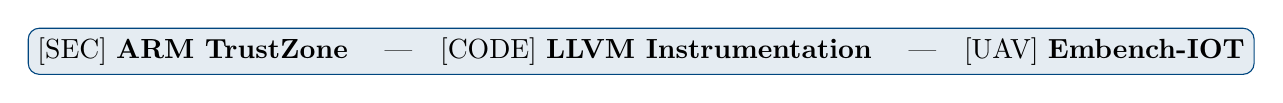
\begin{tikzpicture}
            \node[draw=droneblue, fill=droneblue!10, rounded corners=4pt,
                  minimum width=10cm, minimum height=0.55cm] {%
                [SEC] \textbf{ARM TrustZone} \quad|\quad
                [CODE] \textbf{LLVM Instrumentation} \quad|\quad
                [UAV] \textbf{Embench-IOT}
            };
        \end{tikzpicture}
    \end{center}
\end{frame}

% ─── Outline ──────────────────────────────────────────────────────────────────
\begin{frame}{Outline}
    \tableofcontents
\end{frame}

% ══════════════════════════════════════════════════════════════════════════════
\section{Motivation \& Introduction}
% ══════════════════════════════════════════════════════════════════════════════

\begin{frame}{Why Do We Care About UAV Security?}
    \begin{columns}[T]
        \begin{column}{0.50\textwidth}
            \begin{defbox}{UAVs Are Everywhere}
                \scriptsize Unmanned Aerial Vehicles are now used in:
                \begin{itemize}\scriptsize
                    \item[$>$] Military reconnaissance \& surveillance
                    \item[$>$] Package delivery (Amazon, Zomato)
                    \item[$>$] Precision agriculture
                    \item[$>$] Search \& rescue operations
                    \item[$>$] Infrastructure inspection
                \end{itemize}
            \end{defbox}
            \vspace{3pt}
            \begin{warnbox}{The Problem}
                \scriptsize UAVs run \textbf{safety-critical} software
                \textbf{autonomously} with little human supervision.
                A compromised drone can crash, be hijacked, or cause physical harm.
                Existing flight-control stacks have \textbf{no runtime integrity guarantees}.
            \end{warnbox}
        \end{column}
        \begin{column}{0.46\textwidth}
            \begin{center}
            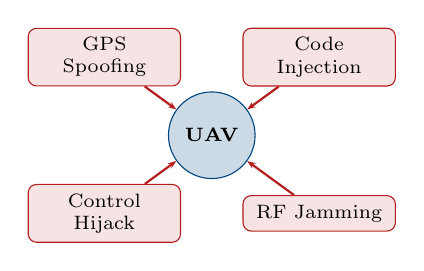
\begin{tikzpicture}[scale=0.62]
                \node[draw=droneblue, fill=droneblue!20, circle, minimum size=1.1cm,
                      font=\scriptsize\bfseries] (drone) at (0,0) {UAV};
                \node[draw=secred, fill=secred!12, rounded corners=3pt,
                      font=\scriptsize, text width=1.7cm, align=center] (gps)
                      at (-2.2, 1.6) {GPS Spoofing};
                \node[draw=secred, fill=secred!12, rounded corners=3pt,
                      font=\scriptsize, text width=1.7cm, align=center] (code)
                      at ( 2.2, 1.6) {Code Injection};
                \node[draw=secred, fill=secred!12, rounded corners=3pt,
                      font=\scriptsize, text width=1.7cm, align=center] (ctl)
                      at (-2.2,-1.6) {Control Hijack};
                \node[draw=secred, fill=secred!12, rounded corners=3pt,
                      font=\scriptsize, text width=1.7cm, align=center] (rf)
                      at ( 2.2,-1.6) {RF Jamming};
                \draw[-{Stealth[length=3pt]}, secred, thick] (gps) -- (drone);
                \draw[-{Stealth[length=3pt]}, secred, thick] (code) -- (drone);
                \draw[-{Stealth[length=3pt]}, secred, thick] (ctl)  -- (drone);
                \draw[-{Stealth[length=3pt]}, secred, thick] (rf)   -- (drone);
            \end{tikzpicture}
            \end{center}
            \vspace{2pt}
            \centering\scriptsize\textbf{Attack surface of a modern UAV}
        \end{column}
    \end{columns}
\end{frame}

% ─────────────────────────────────────────────────────────────────────────────
\begin{frame}{What Is Our Focus?}
    \begin{center}
        \large\textbf{Can we \emph{verify} that a UAV's flight-control software
        is executing exactly as intended — at runtime?}
    \end{center}
    \vspace{8pt}
    \begin{columns}[T]
        \begin{column}{0.32\textwidth}
            \begin{greenbox}{[FIND] Integrity Verification}
                We want to \textbf{detect} any deviation from the expected
                execution path — even if the attacker has code-level access.
            \end{greenbox}
        \end{column}
        \begin{column}{0.32\textwidth}
            \begin{defbox}{[CHART] Performance Benchmarking}
                Attestation adds overhead. We must measure \textbf{how much}
                to assess real-world deployability on embedded hardware.
            \end{defbox}
        \end{column}
        \begin{column}{0.32\textwidth}
            \begin{warnbox}{[SCALE] Schemes Compared}
                We compare three attestation schemes:
                \begin{itemize}
                    \item Branch Counter
                    \item OAT (count-only)
                    \item C-FLAT (full TEE)
                \end{itemize}
            \end{warnbox}
        \end{column}
    \end{columns}
\end{frame}

% ══════════════════════════════════════════════════════════════════════════════
\section{Background}
% ══════════════════════════════════════════════════════════════════════════════

\begin{frame}{Background: Control-Flow Attestation (CFA) — The Big Picture}
    \begin{defbox}{What is Attestation?}
        \textbf{Attestation} is the process by which a \emph{prover} (the UAV)
        convinces a \emph{verifier} (ground station) that its software is running
        correctly and has not been tampered with.
    \end{defbox}
    \vspace{6pt}

    \begin{center}
    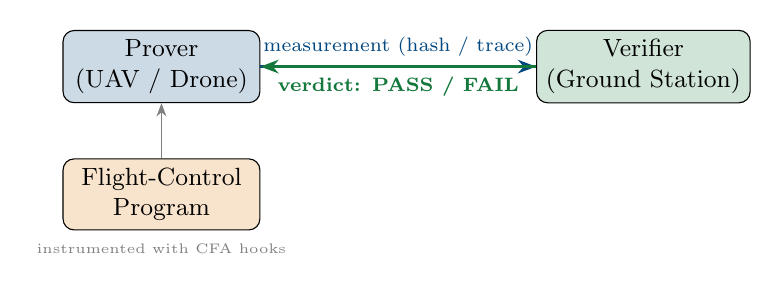
\begin{tikzpicture}[node distance=0.6cm and 1.8cm,
        box/.style={draw, rounded corners=4pt, minimum width=2.5cm,
                    minimum height=0.8cm, align=center, font=\small}]
        \node[box, fill=droneblue!20] (prover) {Prover\\(UAV / Drone)};
        \node[box, fill=trustgreen!20, right=3.5cm of prover] (verifier)
              {Verifier\\(Ground Station)};
        \node[box, fill=warnorange!20, below=0.7cm of prover] (program)
              {Flight-Control\\Program};

        \draw[-{Stealth}, droneblue, thick]
            (prover) -- node[above, font=\scriptsize]
            {measurement (hash / trace)} (verifier);
        \draw[-{Stealth}, trustgreen, thick]
            (verifier) -- node[below, font=\scriptsize]
            {\textbf{verdict: PASS / FAIL}} (prover);
        \draw[-{Stealth}, gray] (program) -- (prover);

        \node[font=\tiny, text=gray, below=0.05cm of program]
              {instrumented with CFA hooks};
    \end{tikzpicture}
    \end{center}
    \vspace{4pt}

    \textbf{Control-Flow Attestation} specifically verifies that the program
    followed a \emph{legitimate control-flow path} — it cannot be fooled by
    code-reuse attacks (ROP/JOP) that only jump between valid code fragments.
\end{frame}

% ─────────────────────────────────────────────────────────────────────────────
\begin{frame}{Background: ARM TrustZone}
    \begin{columns}[T]
        \begin{column}{0.54\textwidth}
            \begin{defbox}{What is TrustZone?}
                \scriptsize ARM TrustZone is a \textbf{hardware security extension} that
                divides the processor into two isolated worlds:
                \begin{itemize}\scriptsize
                    \item \textbf{Normal World (REE):} Runs Linux, ArduCopter,
                          ROS~2 --- untrusted application code.
                    \item \textbf{Secure World (TEE):} Runs OP-TEE OS ---
                          stores secrets, performs attestation; isolated
                          from Normal World by hardware.
                \end{itemize}
                A hardware \texttt{NS} bit enforces the separation.
            \end{defbox}
            \vspace{3pt}
            \begin{warnbox}{Why Does CFA Need TrustZone?}
                \scriptsize An attacker controlling Normal World can forge a software
                attestation log. Only a \textbf{hardware root-of-trust}
                (TrustZone TEE) produces unforgeable measurements.
            \end{warnbox}
        \end{column}
        \begin{column}{0.43\textwidth}
            \begin{center}
            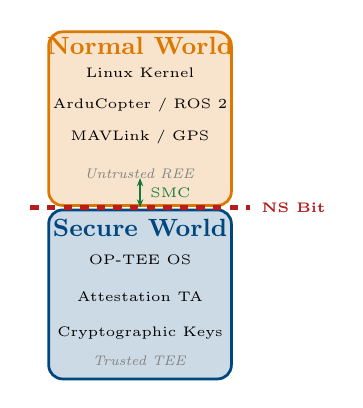
\begin{tikzpicture}[scale=0.58]
                \draw[fill=warnorange!20, draw=warnorange, rounded corners=5pt, line width=1pt]
                      (-2.0, 0) rectangle (2.0, 3.8);
                \node[font=\small\bfseries, text=warnorange] at (0, 3.5) {Normal World};
                \node[font=\tiny] at (0, 2.9) {Linux Kernel};
                \node[font=\tiny] at (0, 2.2) {ArduCopter / ROS~2};
                \node[font=\tiny] at (0, 1.5) {MAVLink / GPS};
                \node[font=\tiny, color=gray] at (0, 0.7) {\textit{Untrusted REE}};

                \draw[fill=droneblue!20, draw=droneblue, rounded corners=5pt, line width=1pt]
                      (-2.0,-3.8) rectangle (2.0,-0.1);
                \node[font=\small\bfseries, text=droneblue] at (0,-0.5) {Secure World};
                \node[font=\tiny] at (0,-1.2) {OP-TEE OS};
                \node[font=\tiny] at (0,-2.0) {Attestation TA};
                \node[font=\tiny] at (0,-2.8) {Cryptographic Keys};
                \node[font=\tiny, color=gray] at (0,-3.4) {\textit{Trusted TEE}};

                \draw[line width=2pt, secred, dashed]
                      (-2.4,-0.05) -- (2.4,-0.05)
                      node[right, font=\tiny\bfseries, text=secred] {NS Bit};
                \draw[{Stealth[length=3pt]}-{Stealth[length=3pt]}, trustgreen, thick]
                      (0,-0.05) -- node[right, font=\tiny] {SMC} (0, 0.6);
            \end{tikzpicture}
            \end{center}
        \end{column}
    \end{columns}
\end{frame}

% ─────────────────────────────────────────────────────────────────────────────
\begin{frame}{Background: OP-TEE}
    \begin{columns}[T]
        \begin{column}{0.52\textwidth}
            \begin{defbox}{OP-TEE — Open Portable Trusted Execution Env.}
                OP-TEE is an \textbf{open-source TEE} from Linaro that runs in
                ARM TrustZone's Secure World.
                \begin{itemize}
                    \item Implements the \textbf{GlobalPlatform TEE API}
                    \item Hosts small programs called
                          \textbf{Trusted Applications (TAs)}
                    \item Normal World talks to it via \texttt{libteec} + SMC
                    \item Provides secure storage, crypto primitives, and
                          attestation logic
                \end{itemize}
            \end{defbox}
            \vspace{4pt}
            \textbf{In our work:} The C-FLAT Trusted Application (TA) lives
            inside OP-TEE.  It receives control-flow hashes from the instrumented
            benchmark and validates them against a \emph{reference CFG}.
        \end{column}
        \begin{column}{0.45\textwidth}
            \begin{center}
            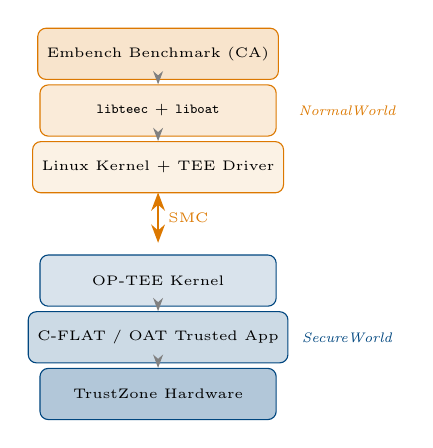
\begin{tikzpicture}[scale=0.8,
                box/.style={draw, rounded corners=3pt, minimum width=3cm,
                            minimum height=0.65cm, align=center, font=\tiny}]
                \node[box, fill=warnorange!20, draw=warnorange] (app)
                      at (0, 3.0) {Embench Benchmark (CA)};
                \node[box, fill=warnorange!15, draw=warnorange] (lib)
                      at (0, 2.1) {\texttt{libteec} + \texttt{liboat}};
                \node[box, fill=warnorange!10, draw=warnorange] (kern)
                      at (0, 1.2) {Linux Kernel + TEE Driver};

                \draw[{Stealth}-{Stealth}, thick, warnorange]
                      (0, 0.8) -- node[right, font=\tiny]{SMC} (0, 0.0);

                \node[box, fill=droneblue!15, draw=droneblue] (optee)
                      at (0,-0.6) {OP-TEE Kernel};
                \node[box, fill=droneblue!20, draw=droneblue] (ta)
                      at (0,-1.5) {C-FLAT / OAT Trusted App};
                \node[box, fill=droneblue!30, draw=droneblue] (hw)
                      at (0,-2.4) {TrustZone Hardware};

                \draw[-{Stealth}, gray, thin] (app) -- (lib);
                \draw[-{Stealth}, gray, thin] (lib) -- (kern);
                \draw[-{Stealth}, gray, thin] (optee) -- (ta);
                \draw[-{Stealth}, gray, thin] (ta) -- (hw);

                \node[font=\tiny\itshape, text=warnorange] at (3.0, 2.1)
                      {Normal\\World};
                \node[font=\tiny\itshape, text=droneblue] at (3.0,-1.5)
                      {Secure\\World};
            \end{tikzpicture}
            \end{center}
        \end{column}
    \end{columns}
\end{frame}

% ─────────────────────────────────────────────────────────────────────────────
\begin{frame}{Background: LLVM \& Compiler Instrumentation}
    \begin{columns}[T]
        \begin{column}{0.50\textwidth}
            \begin{defbox}{Why LLVM?}
                LLVM is a modern compiler framework with a \textbf{pass plugin}
                system.  We write custom \emph{LLVM passes} that automatically
                insert attestation hooks into any C program at compile time.
                \begin{itemize}
                    \item \textbf{No source changes needed} — works on
                          unmodified benchmark C files
                    \item Operates on \textbf{LLVM~IR} (intermediate
                          representation) — architecture-neutral
                    \item Cross-compile the instrumented IR for
                          \textbf{AArch64} (ARM) with a single flag
                \end{itemize}
            \end{defbox}
        \end{column}
        \begin{column}{0.48\textwidth}
            \begin{center}
            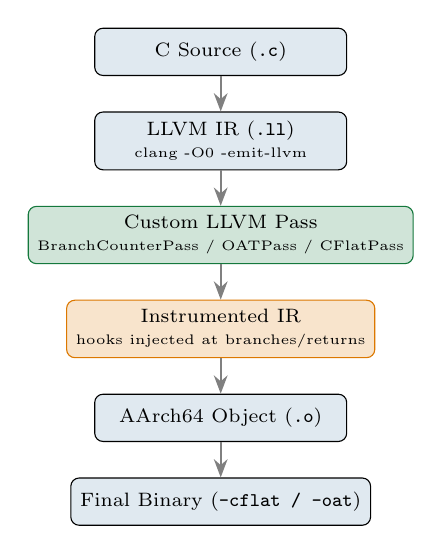
\begin{tikzpicture}[node distance=0.45cm,
                stage/.style={draw, rounded corners=3pt, fill=droneblue!12,
                              minimum width=3.2cm, minimum height=0.6cm,
                              align=center, font=\scriptsize}]
                \node[stage] (src) {C Source (\texttt{.c})};
                \node[stage, below=of src] (ir) {LLVM IR (\texttt{.ll})\\
                      {\tiny clang -O0 -emit-llvm}};
                \node[stage, below=of ir, fill=trustgreen!20, draw=trustgreen]
                      (pass) {Custom LLVM Pass\\
                      {\tiny BranchCounterPass / OATPass / CFlatPass}};
                \node[stage, below=of pass, fill=warnorange!20, draw=warnorange]
                      (inst) {Instrumented IR\\
                      {\tiny hooks injected at branches/returns}};
                \node[stage, below=of inst] (obj) {AArch64 Object (\texttt{.o})};
                \node[stage, below=of obj] (bin)
                      {Final Binary (\texttt{-cflat / -oat})};

                \draw[-{Stealth}, thick, gray] (src) -- (ir);
                \draw[-{Stealth}, thick, gray] (ir) -- (pass);
                \draw[-{Stealth}, thick, gray] (pass) -- (inst);
                \draw[-{Stealth}, thick, gray] (inst) -- (obj);
                \draw[-{Stealth}, thick, gray] (obj) -- (bin);
            \end{tikzpicture}
            \end{center}
        \end{column}
    \end{columns}
\end{frame}

% ══════════════════════════════════════════════════════════════════════════════
\section{Threat Model}
% ══════════════════════════════════════════════════════════════════════════════

\begin{frame}{Threat Model}
    \begin{columns}[T]
        \begin{column}{0.48\textwidth}
            \begin{warnbox}{[THREAT] Attacker Capabilities}
                \begin{itemize}
                    \item Full control of \textbf{Normal World} (Linux + apps)
                    \item Can modify flight-controller firmware or
                          inject malicious waypoints
                    \item Can perform \textbf{GPS spoofing} — feed fake
                          coordinates to fool navigation
                    \item Can launch \textbf{code-reuse attacks}
                          (ROP/JOP) in Normal World
                    \item \textbf{Cannot} compromise TrustZone's Secure World
                    \item \textbf{Cannot} tamper with hardware root-of-trust
                \end{itemize}
            \end{warnbox}
        \end{column}
        \begin{column}{0.48\textwidth}
            \begin{greenbox}{[SEC] What We Protect}
                \begin{itemize}
                    \item \textbf{Control-flow integrity} of the
                          flight-control program
                    \item \textbf{Attestation evidence} (stored in Secure World,
                          signed with TEE keys)
                    \item \textbf{Reference CFG} (Control-Flow Graph) of the
                          expected execution path
                \end{itemize}
            \end{greenbox}
            \vspace{6pt}
            \begin{defbox}{[WARN] Primary Attack Scenario}
                An adversary injects a payload that alters the UAV's flight
                path (via GPS spoofing or memory corruption).
                The CFA scheme must \textbf{detect the deviation} and report
                it to the ground station.
            \end{defbox}
        \end{column}
    \end{columns}
\end{frame}

% ══════════════════════════════════════════════════════════════════════════════
\section{Integrity Verification \& Attestation Schemes}
% ══════════════════════════════════════════════════════════════════════════════

\begin{frame}{What Is Control-Flow Integrity (CFI) Verification?}
    \begin{columns}[T]
        \begin{column}{0.40\textwidth}
            \begin{defbox}{The Key Insight}
                \scriptsize Every program follows a finite set of valid
                \textbf{control-flow paths}.
                An attack \emph{must} deviate from these paths.
                So verifying the path $\equiv$ verifying integrity.
            \end{defbox}
            \vspace{6pt}
            \begin{greenbox}{How CFA Works}
                \scriptsize
                \textbf{At build time:} extract the valid Control-Flow Graph (CFG).\\[3pt]
                \textbf{At runtime:} record executed path as a measurement.\\[3pt]
                \textbf{At verification:} compare measurement to the CFG.\\[3pt]
                \textcolor{secred}{\textbf{Mismatch $\Rightarrow$ Attack detected.}}
            \end{greenbox}
        \end{column}
        \begin{column}{0.56\textwidth}
            \begin{center}
            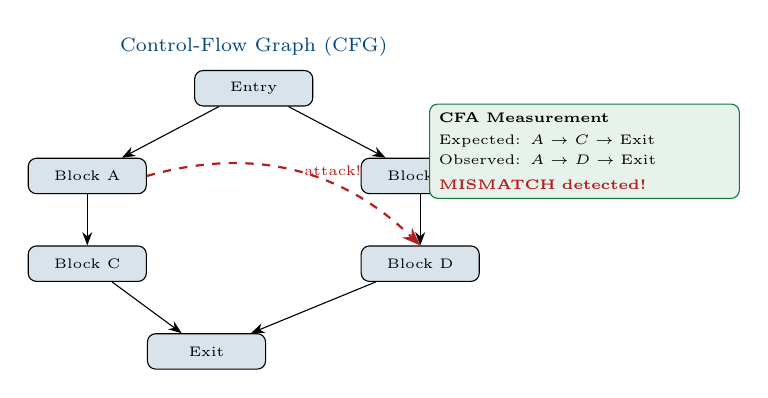
\begin{tikzpicture}[node distance=0.75cm,
                bb/.style={draw, rounded corners=3pt, fill=droneblue!15,
                           minimum width=1.5cm, minimum height=0.45cm,
                           align=center, font=\tiny}]
                \node[bb] (entry) {Entry};
                \node[bb, below left=0.65cm and 0.6cm of entry]  (b1) {Block A};
                \node[bb, below right=0.65cm and 0.6cm of entry] (b2) {Block B};
                \node[bb, below=0.65cm of b1] (b3) {Block C};
                \node[bb, below=0.65cm of b2] (b4) {Block D};
                \node[bb, below right=0.65cm and 0.0cm of b3]    (exit) {Exit};

                \draw[-{Stealth}] (entry)--(b1); \draw[-{Stealth}] (entry)--(b2);
                \draw[-{Stealth}] (b1)--(b3);    \draw[-{Stealth}] (b2)--(b4);
                \draw[-{Stealth}] (b3)--(exit);  \draw[-{Stealth}] (b4)--(exit);

                \draw[-{Stealth}, secred, thick, dashed]
                      (b1.east) to[bend left=30]
                      node[right, font=\tiny, text=secred] {attack!} (b4.north);

                \node[font=\scriptsize, text=droneblue, above=0.05cm of entry]
                      {Control-Flow Graph (CFG)};

                \node[draw=trustgreen, fill=trustgreen!10, rounded corners=3pt,
                      font=\tiny, align=left, minimum width=3.8cm, text width=3.7cm]
                      at (4.2, -0.8) {
                      \textbf{CFA Measurement}\\[2pt]
                      Expected: $A \to C \to \text{Exit}$\\[1pt]
                      Observed: $A \to D \to \text{Exit}$\\[3pt]
                      \textcolor{secred}{\textbf{MISMATCH detected!}}};
            \end{tikzpicture}
            \end{center}
        \end{column}
    \end{columns}
\end{frame}

% ─────────────────────────────────────────────────────────────────────────────
\begin{frame}{C-FLAT Count-Only: Instrumentation Scope}
    \begin{columns}[T]
        \begin{column}{0.48\textwidth}
            \begin{defbox}{C-FLAT instruments ALL control-flow events}
                \scriptsize
                \renewcommand{\arraystretch}{1.3}
                \begin{tabular}{ll}
                    \textbf{Event} & \textbf{Hooks} \\
                    \hline
                    Conditional branches  & 1 per branch \\
                    Unconditional branches & 1 per branch \\
                    Loop headers          & 1 per back-edge \\
                    Direct calls          & 1 per call \\
                    Returns               & 1 per return \\
                    Init + Finalize       & +2 fixed \\
                \end{tabular}
            \end{defbox}
            \vspace{4pt}
            \begin{warnbox}{OAT vs C-FLAT: Key Difference}
                \scriptsize OAT (Smin) skips \textbf{unconditional branches},
                \textbf{loop headers}, and \textbf{direct calls} --- targeting only
                the minimum set needed for secure attestation.\\[3pt]
                C-FLAT includes all of these for \textbf{full path coverage}.
            \end{warnbox}
        \end{column}
        \begin{column}{0.48\textwidth}
            \begin{greenbox}{Measured Results (AArch64)}
                \scriptsize
                \renewcommand{\arraystretch}{1.2}
                \begin{tabular}{lr}
                    \textbf{Benchmark} & \textbf{CFLAT switches} \\
                    \hline
                    aha-mont64     & 857.8M \\
                    crc32          & 871.9M \\
                    primecount     & 1,607.2M \\
                    sglib-combined & 1,461.7M \\
                    nbody          &    17.3M \\
                    cubic          &     2.0M \\
                \end{tabular}
            \end{greenbox}
            \vspace{4pt}
            \begin{defbox}{Why Count-Only?}
                \scriptsize \texttt{min\_libcflat.c} replaces \texttt{libteec}/SMC
                with a simple counter --- \textbf{no TEE required}.
                Measured counts give an upper bound for full C-FLAT
                deployment cost on OP-TEE.
            \end{defbox}
        \end{column}
    \end{columns}
\end{frame}

% ══════════════════════════════════════════════════════════════════════════════
\section{Why Benchmarking?}
% ══════════════════════════════════════════════════════════════════════════════

\begin{frame}{Why Do We Need Performance Benchmarking?}
    \begin{columns}[T]
        \begin{column}{0.50\textwidth}
            \begin{defbox}{UAV Real-Time Constraints}
                \scriptsize UAV flight-control loops run at \textbf{fixed frequencies}
                (400~Hz attitude, 50~Hz position).
                Attestation that breaks these deadlines is
                \textbf{a safety problem, not just a performance problem.}
                \vspace{2pt}

                Attestation must not:
                \begin{itemize}\scriptsize
                    \item Delay motor commands past the control loop period
                    \item Cause jitter in sensor fusion pipelines
                    \item Block GPS or IMU data processing
                \end{itemize}
            \end{defbox}
            \vspace{3pt}
            \textbf{\scriptsize Benchmarking lets us ask:}
            \begin{enumerate}\scriptsize
                \item Which code regions fit within the real-time deadline?
                \item Does OAT or C-FLAT suit the UAV timing budget?
                \item Where to use lightweight counting vs.\ full TEE?
            \end{enumerate}
        \end{column}
        \begin{column}{0.47\textwidth}
            \begin{defbox}{Embench-IOT: Why This Suite?}
                \scriptsize Standard embedded benchmark suite for IoT workloads.
                \begin{itemize}\scriptsize
                    \item 15 benchmarks: crypto, math, sorting, strings
                    \item Self-contained with \texttt{main()} --- easy to instrument
                    \item Used in CFA papers (OAT, BLAST, Tiny-CFA)
                    \item Cross-compiles cleanly to AArch64
                \end{itemize}
            \end{defbox}
            \vspace{3pt}
            \begin{greenbox}{Security vs.\ Real-Time: The Core Tradeoff}
                \scriptsize More instrumentation $\Rightarrow$ stronger attestation,
                but more control-loop interruptions.
                Benchmarking \textbf{quantifies} this tradeoff for
                principled deployment decisions.
            \end{greenbox}
        \end{column}
    \end{columns}
\end{frame}

% ══════════════════════════════════════════════════════════════════════════════
\section{Implementation}
% ══════════════════════════════════════════════════════════════════════════════

\begin{frame}{Implementation Overview}
\begin{center}
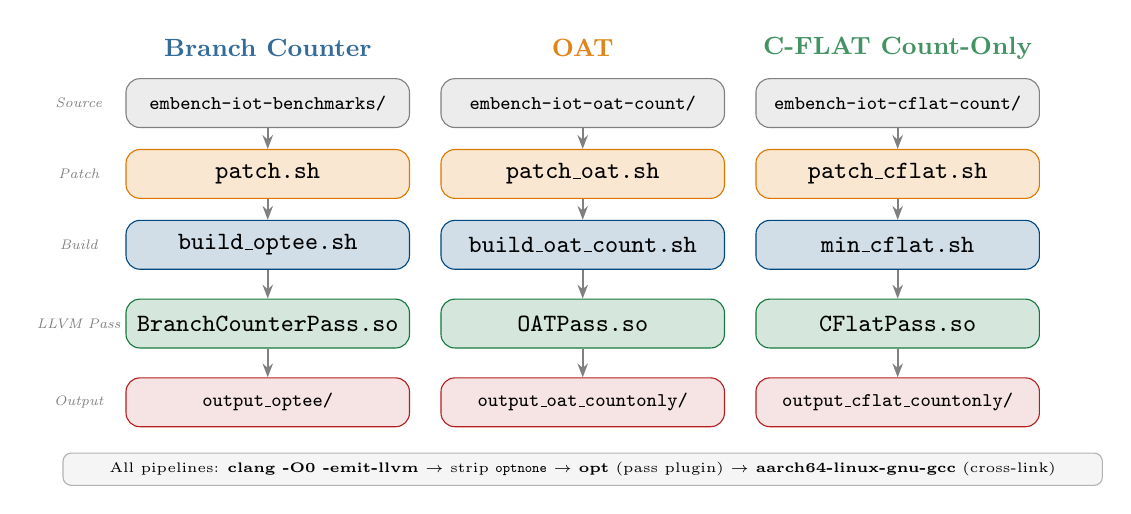
\begin{tikzpicture}[
    lane/.style={draw, rounded corners=5pt, fill=#1, minimum width=3.6cm,
                 minimum height=0.62cm, align=center, font=\small},
    laneS/.style={draw, rounded corners=5pt, fill=#1, minimum width=3.6cm,
                 minimum height=0.62cm, align=center, font=\scriptsize},
    arr/.style={-{Stealth[length=5pt]}, thick, gray},
    hdr/.style={font=\small\bfseries, text=#1}
]

%% ── Column headers ─────────────────────────────────────────────────────
\node[hdr=droneblue!80]   at (-4.0, 3.6) {Branch Counter};
\node[hdr=warnorange!90]  at ( 0.0, 3.6) {OAT};
\node[hdr=trustgreen!80]  at ( 4.0, 3.6) {C-FLAT Count-Only};

%% ── Row labels (left margin) ───────────────────────────────────────────
\node[font=\tiny\itshape, text=gray, align=right] at (-6.4, 2.9) {Source};
\node[font=\tiny\itshape, text=gray, align=right] at (-6.4, 2.0) {Patch};
\node[font=\tiny\itshape, text=gray, align=right] at (-6.4, 1.1) {Build};
\node[font=\tiny\itshape, text=gray, align=right] at (-6.4, 0.1) {LLVM Pass};
\node[font=\tiny\itshape, text=gray, align=right] at (-6.4,-0.9) {Output};

%% ── Source trees ───────────────────────────────────────────────────────
\node[laneS=gray!15, draw=gray]          (s1) at (-4.0, 2.9)
      {\texttt{embench-iot-benchmarks/}};
\node[laneS=gray!15, draw=gray]          (s2) at ( 0.0, 2.9)
      {\texttt{embench-iot-oat-count/}};
\node[laneS=gray!15, draw=gray]          (s3) at ( 4.0, 2.9)
      {\texttt{embench-iot-cflat-count/}};

%% ── Patch scripts ──────────────────────────────────────────────────────
\node[lane=warnorange!18, draw=warnorange] (p1) at (-4.0, 2.0)
      {\texttt{patch.sh}};
\node[lane=warnorange!18, draw=warnorange] (p2) at ( 0.0, 2.0)
      {\texttt{patch\_oat.sh}};
\node[lane=warnorange!18, draw=warnorange] (p3) at ( 4.0, 2.0)
      {\texttt{patch\_cflat.sh}};

%% ── Build scripts ──────────────────────────────────────────────────────
\node[lane=droneblue!18, draw=droneblue]   (b1) at (-4.0, 1.1)
      {\texttt{build\_optee.sh}};
\node[lane=droneblue!18, draw=droneblue]   (b2) at ( 0.0, 1.1)
      {\texttt{build\_oat\_count.sh}};
\node[lane=droneblue!18, draw=droneblue]   (b3) at ( 4.0, 1.1)
      {\texttt{min\_cflat.sh}};

%% ── LLVM passes ────────────────────────────────────────────────────────
\node[lane=trustgreen!18, draw=trustgreen] (lp1) at (-4.0, 0.1)
      {\texttt{BranchCounterPass.so}};
\node[lane=trustgreen!18, draw=trustgreen] (lp2) at ( 0.0, 0.1)
      {\texttt{OATPass.so}};
\node[lane=trustgreen!18, draw=trustgreen] (lp3) at ( 4.0, 0.1)
      {\texttt{CFlatPass.so}};

%% ── Outputs ────────────────────────────────────────────────────────────
\node[laneS=secred!12, draw=secred]        (o1) at (-4.0,-0.9)
      {\texttt{output\_optee/}};
\node[laneS=secred!12, draw=secred]        (o2) at ( 0.0,-0.9)
      {\texttt{output\_oat\_countonly/}};
\node[laneS=secred!12, draw=secred]        (o3) at ( 4.0,-0.9)
      {\texttt{output\_cflat\_countonly/}};

%% ── Vertical arrows within each lane ──────────────────────────────────
\draw[arr] (s1) -- (p1); \draw[arr] (p1) -- (b1); \draw[arr] (b1) -- (lp1); \draw[arr] (lp1) -- (o1);
\draw[arr] (s2) -- (p2); \draw[arr] (p2) -- (b2); \draw[arr] (b2) -- (lp2); \draw[arr] (lp2) -- (o2);
\draw[arr] (s3) -- (p3); \draw[arr] (p3) -- (b3); \draw[arr] (b3) -- (lp3); \draw[arr] (lp3) -- (o3);

%% ── Shared runtime note ────────────────────────────────────────────────
\node[draw=gray!60, fill=gray!8, rounded corners=3pt,
      font=\tiny, align=center, minimum width=13.2cm]
      at (0,-1.75)
      {All pipelines: \textbf{clang -O0 -emit-llvm} $\to$
       strip \texttt{optnone} $\to$ \textbf{opt} (pass plugin) $\to$
       \textbf{aarch64-linux-gnu-gcc} (cross-link)};
\end{tikzpicture}
\end{center}
\end{frame}

% ─────────────────────────────────────────────────────────────────────────────
\begin{frame}[fragile]{The LLVM Instrumentation Pipeline (Step by Step)}
    \begin{columns}[T]
        \begin{column}{0.50\textwidth}
            \textbf{\scriptsize Pipeline for every benchmark:}
            \vspace{1pt}
            \begin{enumerate}\scriptsize
                \item \textbf{Generate LLVM IR} at \texttt{-O0}:
                      \begin{lstlisting}[style=bashstyle]
clang -O0 -S -emit-llvm \
  --target=aarch64-linux-gnu \
  mont64.c -o mont64.ll
                      \end{lstlisting}
                \item \textbf{Strip \texttt{optnone}} so passes run:
                      \begin{lstlisting}[style=bashstyle]
opt -strip-debug -S mont64.ll | \
  sed 's/optnone/noinline/g' \
  > mont64_stripped.ll
                      \end{lstlisting}
                \item \textbf{Run pass plugin:}
                      \begin{lstlisting}[style=bashstyle]
opt -load-pass-plugin=OATPass.so \
    -passes="oat-pass" \
    -S mont64.ll -o mont64_inst.ll
                      \end{lstlisting}
                \item \textbf{Compile + cross-link:}
                      \begin{lstlisting}[style=bashstyle]
clang -c mont64_inst.ll -o mont64.o
aarch64-linux-gnu-gcc \
  mont64.o liboat_count_only.o \
  -o mont64-oat
                      \end{lstlisting}
            \end{enumerate}
        \end{column}
        \begin{column}{0.47\textwidth}
            \textbf{\scriptsize What each pass injects:}
            \vspace{2pt}

            \begin{defbox}{BranchCounterPass}
                \scriptsize \texttt{increment\_branch(id)} at every branch edge.
                Counts branch frequency --- lightweight baseline.
            \end{defbox}
            \vspace{2pt}
            \begin{warnbox}{OATPass (Smin)}
                \scriptsize \texttt{\_\_oat\_log(val)} at cond.\ branch targets,\\
                \texttt{\_\_oat\_log\_indirect(addr)} at indirect calls,\\
                \texttt{\_\_oat\_func\_exit(id)} at returns.\\
                \textit{Direct calls excluded per OAT paper.}
            \end{warnbox}
            \vspace{2pt}
            \begin{greenbox}{CFlatPass}
                \scriptsize \texttt{cflat\_record(id)} at cond.\ branches, uncond.\
                branches, loop headers, calls, returns.
                Full path coverage for count-only mode.
            \end{greenbox}
        \end{column}
    \end{columns}
\end{frame}

% ─────────────────────────────────────────────────────────────────────────────
\begin{frame}[fragile]{Patching the Benchmark Source Files}
    \texttt{patch\_*.sh} scripts use \texttt{sed} to inject runtime hooks into Embench C sources.
    \vspace{4pt}
    \begin{columns}[T]
        \begin{column}{0.32\textwidth}
            \begin{defbox}{\texttt{patch.sh} (Branch Counter)}
                \begin{lstlisting}[style=cstyle, language=C]
// After warm_caches():
init_branch_stats();

// Before verify_benchmark():
print_branch_stats();
                \end{lstlisting}
            \end{defbox}
        \end{column}
        \begin{column}{0.32\textwidth}
            \begin{warnbox}{\texttt{patch\_oat.sh} (OAT)}
                \begin{lstlisting}[style=cstyle, language=C]
// Before benchmark():
__oat_init();

// Before verify_benchmark():
__oat_print_proof();
                \end{lstlisting}
                \tiny warm\_caches() \textbf{excluded} from OAT scope.
            \end{warnbox}
        \end{column}
        \begin{column}{0.32\textwidth}
            \begin{greenbox}{\texttt{patch\_cflat.sh} (C-FLAT)}
                \begin{lstlisting}[style=cstyle, language=C]
// Before verify_benchmark():
cflat_finalize_and_print();
                \end{lstlisting}
                \tiny \texttt{min\_libcflat} counts locally,\\no TEE dependency.
            \end{greenbox}
        \end{column}
    \end{columns}
    \vspace{8pt}
    \begin{columns}[T]
        \begin{column}{0.32\textwidth}
            \centering\scriptsize
            \textcolor{droneblue}{\textbf{Backup created}} before any patch
        \end{column}
        \begin{column}{0.32\textwidth}
            \centering\scriptsize
            \textcolor{droneblue}{\textbf{Idempotent}} --- skips already-patched files
        \end{column}
        \begin{column}{0.32\textwidth}
            \centering\scriptsize
            \textcolor{droneblue}{\textbf{Pattern-based}} via \texttt{grep} on Embench signatures
        \end{column}
    \end{columns}
\end{frame}

% ══════════════════════════════════════════════════════════════════════════════
\section{Challenges}
% ══════════════════════════════════════════════════════════════════════════════

\begin{frame}{Challenges}
    \begin{columns}[T]
        \begin{column}{0.48\textwidth}
            \begin{warnbox}{Implementation Challenges}
                \begin{enumerate}\scriptsize
                    \item \textbf{\texttt{optnone} attribute} --- Clang inserts
                          this at \texttt{-O0}, blocking all passes.
                          Stripped via \texttt{sed} before instrumentation.
                    \item \textbf{AArch64 cross-compilation} --- Clang emits
                          AArch64 IR; GCC cross-linker produces the final
                          binary against the OP-TEE sysroot.
                    \item \textbf{C-FLAT count-only runtime} --- Full C-FLAT
                          needs \texttt{libteec.so}. We use
                          \texttt{min\_libcflat.c}: a TEE-free counter
                          portable to any AArch64 board.
                    \item \textbf{Math library} (\texttt{-lm}) --- Three
                          benchmarks (\texttt{cubic}, \texttt{nbody},
                          \texttt{st}) require explicit \texttt{-lm} at
                          link time.
                \end{enumerate}
            \end{warnbox}
        \end{column}
        \begin{column}{0.48\textwidth}
            \begin{warnbox}{Research Challenges}
                \begin{enumerate}\scriptsize
                    \item \textbf{Path explosion} --- Loops create exponentially
                          many paths. Addressed using the loop-as-subprogram
                          technique: each iteration hashed as a sub-path.
                    \item \textbf{World-switch overhead} --- High-frequency
                          benchmarks (e.g., \texttt{primecount}: 880M OAT
                          switches) stress real-time UAV constraints.
                    \item \textbf{OAT Smin accuracy} --- Reproducing the exact
                          Smin set requires excluding direct calls and
                          function entries from the pass, matching the paper.
                    \item \textbf{GPS spoofing integration} --- Hooking the
                          NMEA parser in \texttt{gpsd} is the next step for
                          end-to-end UAV attestation.
                \end{enumerate}
            \end{warnbox}
        \end{column}
    \end{columns}
\end{frame}

% ─────────────────────────────────────────────────────────────────────────────
% ══════════════════════════════════════════════════════════════════════════════
\section{Results \& Analysis}
% ══════════════════════════════════════════════════════════════════════════════

\begin{frame}{Measured Results: Branch Counter Statistics (1/2)}
    \begin{center}
    \renewcommand{\arraystretch}{1.15}
    \scriptsize
    \begin{tabular}{lrrrrr}
        \toprule
        \textbf{Benchmark} &
        \textbf{Cond.\ Br.} &
        \textbf{Uncond.\ Br.} &
        \textbf{Loop Hdrs} &
        \textbf{Direct Calls} &
        \textbf{Returns} \\
        \midrule
        aha-mont64    & 384.5M & 456.4M & 189.9M &   8.5M &   8.5M \\
        crc32         & 174.4M & 348.7M & 174.3M & 174.4M & 174.4M \\
        cubic         &   0.7M &   1.0M &   0.3M &   2.0M &   0.2M \\
        edn           & 371.9M & 732.8M & 360.9M &   0.7M &   0.7M \\
        huffbench     & 495.8M & 486.3M & 233.3M &   1.1M &   1.1M \\
        matmult-int   & 406.7M & 794.1M & 387.4M &   0.1M &   0.1M \\
        minver        & 109.3M & 156.0M &  56.6M &   6.1M &   6.1M \\
        nbody         &   6.2M &  10.8M &   4.6M &   1.1M &   0.1M \\
        nettle-aes    &  78.0M & 147.7M &  51.2M &   0.9M &   0.9M \\
        nettle-sha256 &  30.4M & 185.3M &  24.2M &   2.4M &   3.8M \\
        primecount    & 880.2M & 727.0M & 282.3M & $<$0.1M & $<$0.1M \\
        sglib-combined& 680.9M & 627.5M & 147.8M &  76.6M &  76.6M \\
        st            &   9.2M &  18.3M &   9.1M &   8.0M &   7.9M \\
        tarfind       &  80.9M & 114.0M &  48.4M &  36.3M &  36.3M \\
        ud            & 412.4M & 616.3M & 255.7M &   1.5M &   1.5M \\
        \bottomrule
    \end{tabular}
    \end{center}
    \vspace{2pt}
    \centering\tiny All counts in millions (M) $\cdot$ CPU\_MHZ=1000 $\cdot$ AArch64 OP-TEE build
\end{frame}

% ─────────────────────────────────────────────────────────────────────────────
\begin{frame}{Measured Results: CFLAT \& OAT World Switch Counts (2/2)}
    \begin{center}
    \renewcommand{\arraystretch}{1.15}
    \scriptsize
    \begin{tabular}{lrrr}
        \toprule
        \textbf{Benchmark} &
        \textbf{CFLAT Switches} &
        \textbf{OAT Switches} &
        \textbf{Ratio (CFLAT/OAT)} \\
        \midrule
        aha-mont64     &   857.8M &  466.6M & $\times$1.84 \\
        crc32          &   871.9M &  348.8M & $\times$2.50 \\
        cubic          &     2.0M &    0.9M & $\times$2.36 \\
        edn            & 1,106.1M &  372.6M & $\times$2.97 \\
        huffbench      &   984.2M &  602.6M & $\times$1.63 \\
        matmult-int    & 1,201.0M &  406.8M & $\times$2.95 \\
        minver         &   277.5M &  131.0M & $\times$2.12 \\
        nbody          &    17.3M &    6.3M & $\times$2.73 \\
        nettle-aes     &   227.4M &   86.8M & $\times$2.62 \\
        nettle-sha256  &   221.8M &   36.1M & $\times$6.14 \\
        primecount     & 1,607.2M &  880.2M & $\times$1.83 \\
        sglib-combined & 1,461.7M &  990.6M & $\times$1.48 \\
        st             &    43.3M &   17.1M & $\times$2.53 \\
        tarfind        &   267.6M &  142.7M & $\times$1.88 \\
        ud             & 1,031.6M &  437.5M & $\times$2.36 \\
        \bottomrule
    \end{tabular}
    \end{center}
    \vspace{2pt}
    \centering\tiny
    All counts in millions (M) $\cdot$
    CFLAT: cond.+uncond.\ branches, loop headers, calls, returns $\cdot$
    OAT: cond.\ branches, indirect calls, returns (Smin)
\end{frame}

% ─────────────────────────────────────────────────────────────────────────────
\begin{frame}{Key Takeaways from Benchmarking}
    \begin{columns}[T]
        \begin{column}{0.48\textwidth}
            \begin{greenbox}{Finding 1: CFLAT overhead is 1.5--6$\times$ OAT}
                CFLAT world switches are consistently higher than OAT across
                all benchmarks. The ratio ranges from $\times$1.48
                (\texttt{sglib-combined}) to $\times$6.14
                (\texttt{nettle-sha256}), driven by CFLAT also
                instrumenting \textbf{unconditional branches and loop headers}.
            \end{greenbox}
            \vspace{6pt}
            \begin{greenbox}{Finding 2: Loop-heavy benchmarks dominate overhead}
                Benchmarks with large loop counts (e.g.,
                \texttt{primecount}: 282M loop headers,
                \texttt{matmult-int}: 387M) produce the highest switch counts
                --- over \textbf{1.6 billion CFLAT switches} for
                \texttt{primecount}.
            \end{greenbox}
        \end{column}
        \begin{column}{0.48\textwidth}
            \begin{greenbox}{Finding 3: C-FLAT count-only is a safe upper bound}
                \texttt{min\_libcflat} counts all CFlatPass hook sites with
                \textbf{zero TEE dependency}. The measured counts give a
                reliable upper bound for the world-switch cost of a future
                full C-FLAT deployment on OP-TEE.
            \end{greenbox}
            \vspace{6pt}
            \begin{greenbox}{Finding 4: OAT Smin is the lighter practical choice}
                OAT's exclusion of direct calls and loop headers keeps switch
                counts 1.5--6$\times$ lower than CFLAT.
                For UAV real-time constraints, OAT count-only is the most
                deployable scheme across all 15 benchmarks.
            \end{greenbox}
        \end{column}
    \end{columns}
\end{frame}

% ══════════════════════════════════════════════════════════════════════════════
\section{Conclusion \& Future Work}
% ══════════════════════════════════════════════════════════════════════════════

\begin{frame}{Conclusion}
    \begin{center}
        \large\textbf{We built a complete, reproducible CFA benchmarking
        framework for embedded UAV workloads.}
    \end{center}
    \vspace{8pt}
    \begin{columns}[T]
        \begin{column}{0.48\textwidth}
            \textbf{What we built:}
            \begin{itemize}
                \item 3 LLVM pass plugins: Branch Counter, OAT, and C-FLAT (count-only) instrumentation
                \item 4 end-to-end build pipelines (host + AArch64 cross)
                \item 3 patch scripts for automatic runtime hook injection
                \item Complete switch-count data for 15 Embench benchmarks
                \item \texttt{min\_libcflat} runtime: TEE-free C-FLAT count without any libteec dependency
            \end{itemize}
        \end{column}
        \begin{column}{0.48\textwidth}
            \textbf{What we showed:}
            \begin{itemize}
                \item World-switch counts span \textbf{6 orders of magnitude}
                      across benchmarks
                \item C-FLAT count-only and OAT count-only are comparably
                      lightweight and deployable on bare AArch64
                \item Selective attestation of safety-critical UAV subsystems
                      is the recommended deployment strategy
            \end{itemize}
        \end{column}
    \end{columns}
\end{frame}

% ─────────────────────────────────────────────────────────────────────────────
\begin{frame}{Future Work}
    \begin{columns}[T]
        \begin{column}{0.48\textwidth}
            \begin{defbox}{[ROCKET] Near-Term}
                \begin{itemize}
                    \item Deploy C-FLAT on physical Jetson + OP-TEE board
                          and measure real SMC latency
                    \item Hook \texttt{gpsd}'s NMEA parser with CFA to
                          detect GPS spoofing at the kernel/user boundary
                    \item Integrate with \textbf{MAVROS} to attest the
                          GPS $\to$ ROS~2 data pipeline end-to-end
                \end{itemize}
            \end{defbox}
        \end{column}
        \begin{column}{0.48\textwidth}
            \begin{defbox}{[LAB] Research Directions}
                \begin{itemize}
                    \item Evaluate \textbf{BLAST} (Binary-Level Attestation)
                          as a no-recompile alternative
                    \item Implement \textbf{selective CFA} — only attest
                          safety-critical flight-controller functions
                    \item Compare attestation overhead against
                          \textbf{real-time scheduling constraints}
                          (EDF / RMS on ArduCopter loops)
                    \item Extend to multi-UAV swarm attestation scenarios
                \end{itemize}
            \end{defbox}
        \end{column}
    \end{columns}
\end{frame}

% ─────────────────────────────────────────────────────────────────────────────
\begin{frame}
    \begin{center}
        \Huge\textbf{Thank You}\\[16pt]
        \large Questions?\\[24pt]
        \normalsize
        \begin{tabular}{ll}
            [CODE]  & \texttt{OATPass.so / CFlatPass.so / BranchCounterPass.so} \\[4pt]
            [DIR] & \texttt{embench-iot-benchmarks*/} \\[4pt]
            [FILE] & \texttt{output*/oat\_switch\_counts.txt} \\[4pt]
            [SEC] & ARM TrustZone + OP-TEE (Secure World) \\
        \end{tabular}
    \end{center}
\end{frame}

\end{document}